\documentclass{article}
\usepackage{caption}
\usepackage{subcaption}
\usepackage{graphicx}
\usepackage{tikz}
\usepackage{tikzsymbols}
\usetikzlibrary{calc}
\usepackage{float}
\usepackage{pdflscape}
\usepackage{geometry}
\geometry{a4paper, landscape, margin=1cm}
\pagestyle{empty}

\def\centerarc[#1](#2)(#3:#4:#5){\draw[#1] ($(#2)+({#5*cos(#3)},{#5*sin(#3)})$) arc (#3:#4:#5);}

\begin{document}
	\centering
	\begin{figure}[H]
			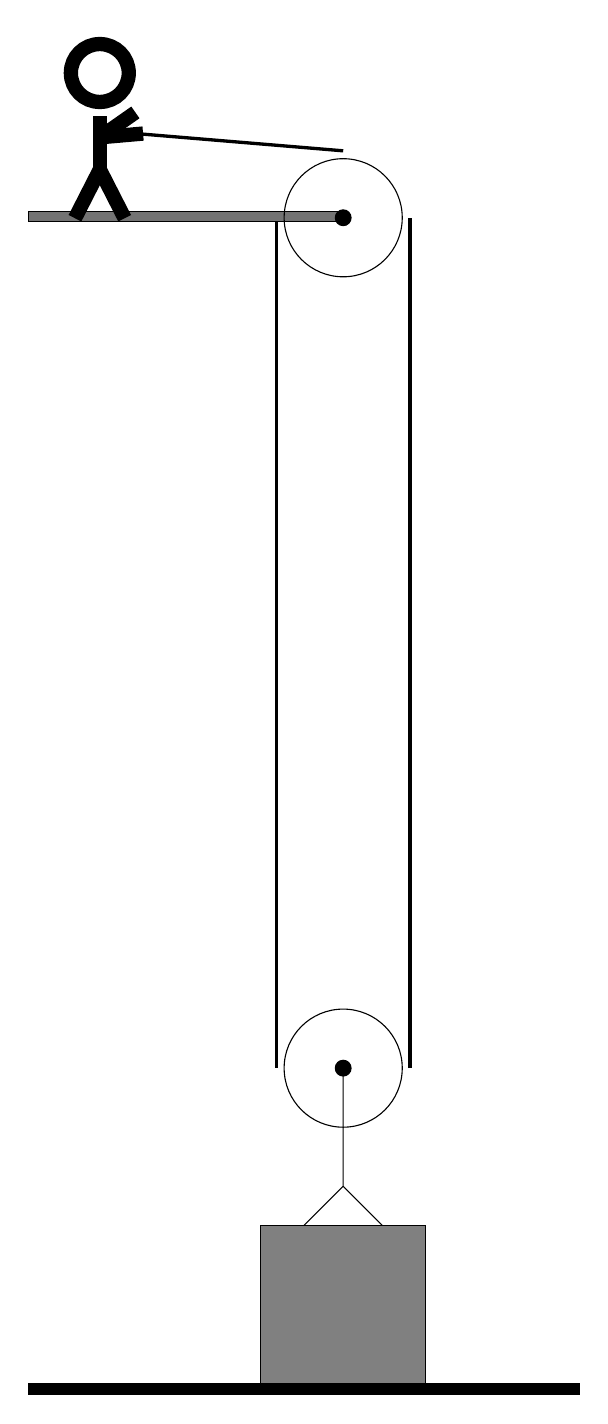
\begin{tikzpicture}
				%%%%% START %%%%%
								
				\draw[fill=black!55] (-2, 11.75) rectangle (2, 11.88);
				
				\draw (2, 1) circle (0.75);
				\draw[fill=black] (2, 1) circle (0.1);
				
				\draw (2, 11.8) circle (0.75);
				\draw[fill=black] (2, 11.8) circle (0.1);
				
				\draw (2, 1) -- (2, -0.5) -- (1.5, -1) -- (2.5, -1) -- (2, -0.5);
				\draw[fill=black!50] (0.95, -1) rectangle (3.05, -3);
				
				\draw[very thick] (1.15, 11.75) -- (1.15, 1);
				\centerarc[very thick](2, 1)(180:360:0.85);
				\draw[very thick](2.85, 1) -- (2.85, 11.8);
				\centerarc[very thick](2, 11.8)(0:90:0.85);
				\draw[very thick](2, 12.65) -- (-1, 12.9);
				
				\node at (-1, 12.9) {\Strichmaxerl[10][-175][35]};
				
				\draw[fill=black] (-2, -3) rectangle (5, -3.15);
				%%%%% END %%%%%
			\end{tikzpicture}
	\end{figure}	
\end{document}